\documentclass[a4paper,12pt]{article}
\setlength{\parindent}{0pt}

\usepackage[ruled,vlined]{algorithm2e}
\usepackage{mlsubmit}
\usepackage{graphicx}

\begin{document}

\initmlsubmision{3} % assignment number
{Utkarsh Gupta}   % your name
{180836}	% your roll number

\begin{mlsolution}

Let the matrix $\vR = \frac{1}{N}\vX\vX^T$. We are given an eigenvector $\vv \in \bR^N$ of $\vR$ (eigenvalue $\lambda_v$) and we have to find eigenvector $\vu \in \bR^D$ of $\vS$ (eigenvalue $\lambda_u$).
From the definition of eigenvectors, we know:
\begin{equation*}
    \frac{1}{N}\vX\vX^T\vv = \lambda_v\vv
\end{equation*}
\begin{equation*}
    \implies \frac{1}{N}\br{\vX^T\vX}\vX^T\vv = \lambda_v\br{\vX^T\vv}
\end{equation*}
\begin{equation*}
    \implies \frac{1}{N}\vS\br{\vX^T\vv} = \lambda_u\br{\vX^T\vv}
\end{equation*}
Thus we have,
\begin{equation*}
    \vu = \vX^T\vv \; \; \& \; \; \lambda_u = \lambda_v
\end{equation*}

We know $D>N$ and $rank(\vS) = rank(\vR) = min(N, D) = N$. $\vS$ is a $D$x$D$ matrix, which means that it has $D$ eigenvectors, $N$ of which can be found using the relation found above and the remaining $D-N$ vectors will be $\pmb{0}$.

The main advantage of using this method is the speed that we gain. Eigendecomposition of a $D$x$D$ (original $\vS$) takes $O(D^3)$ time. Using this method, we can do eigendecomposition of $\vR$ in $O(N^3)$ time and then multiply them with $\vX^T$ in a total time of $O(N^2D)$.
Thus, the total time complexity of this approach is $O(N^3)+O(N^2D) = O(N^2D)$ which is significantly less than the original $O(D^3)$. Hence, this approach will be much faster when $D$ is much larger than $N$.

\end{mlsolution}

\begin{mlsolution}

We are given $\vK$ an $N$ x $M$ matrix that contains the per minute server hit data and $L$ (number of clusters) which is a hyper-parameter. $\pmb{\lambda}$ is an $L$ x $1$ vector, $l^{th}$ entry of which is the Poisson parameter of the $l^{th}$ cluster.

To find the CLL we need:

\begin{equation*}
    p(\vK, \vZ | \pmb{\pi}, \pmb{\lambda}) = \prod\limits_{n=1}^N\sum\limits_{l=1}^L\bs{z_{nl}\;\text{x}\; p(z_n = l)\prod\limits_{m=1}^M\textsc{Poisson}(k_{nm}|\lambda_l)}
\end{equation*}

$\textsc{Poisson}(k|\lambda_l) = \frac{\lambda^k}{k!}e^{-\lambda}$ and $p(z_n = l) = \pi_l$. Since $\vz_n$ is one-hot vector, only one of the $z_{nl}$ is $1$.

\begin{equation*}
    CLL(\vK, \vZ \;|\;\pmb{\pi}, \pmb{\lambda}) = \sum\limits_{n=1}^N\sum\limits_{l=1}^Lz_{nl}\bs{log\;\pi_l + \sum\limits_{m=1}^M\br{k_{nm}log\;\lambda_l - \lambda_l - log\; k_{mn}!}}
\end{equation*}

For solving, we can ignore the objective-independent constants:

\begin{equation}
    CLL(\vK, \vZ \;|\;\pmb{\pi}, \pmb{\lambda}) = \sum\limits_{n=1}^N\sum\limits_{l=1}^Lz_{nl}\bs{log\;\pi_l + \sum\limits_{m=1}^M\br{k_{nm}log\;\lambda_l - \lambda_l}}
\end{equation}

E step:

\begin{equation*}
    \bE\bs{z_{nl}} = 0 \times p(z_{nl}=0\;|\; k_n, \pmb{\pi}, \pmb{\lambda}) + 1 \times p(z_{nl}=1\;|\; k_n, \pmb{\pi}, \pmb{\lambda})
\end{equation*}
\begin{equation*}
    \bE\bs{z_{nl}} = p(z_{nl}=1\;|\; k_n, \pmb{\pi}, \pmb{\lambda}) \propto p(z_n = l\;|\;\pmb{\pi}) \times p(k_n \;|\; z_n=l, \pmb{\lambda})
\end{equation*}
\begin{equation*}
    \implies \bE\bs{z_{nl}} \propto \pi_l \prod\limits_{m=1}^M\frac{\lambda_l^{k_{nm}}}{k_{nm}!}e^{-\lambda_l}
\end{equation*}
\begin{equation}
    \therefore \bE\bs{z_{nl}} = \frac{\pi_l \prod\limits_{m=1}^M\frac{\lambda_l^{k_{nm}}}{k_{nm}!}e^{-\lambda_l}}{\sum\limits_{l=1}^L \pi_l \prod\limits_{m=1}^M\frac{\lambda_l^{k_{nm}}}{k_{nm}!}e^{-\lambda_l}}
\end{equation}

M step:

\begin{equation*}
    \text{arg}\max\limits_{\pmb{\pi}\geq 0, \pmb{\lambda}>0}\bE\bs{CLL(\vK, \vZ \;|\;\pmb{\pi}, \pmb{\lambda})} = \text{arg}\max\limits_{\pmb{\pi}\geq 0, \pmb{\lambda}>0}\sum\limits_{n=1}^N\sum\limits_{l=1}^L\bE\bs{z_{nl}}\bs{log\;\pi_l + \sum\limits_{m=1}^M\br{k_{nm}log\;\lambda_l \pmb{-} \lambda_l}}
\end{equation*}

given $\sum\limits_{l=1}^L\lambda_l =1$. Now, the Lagrangian:

\begin{equation*}
    \text{arg}\max\limits_{\pmb{\pi}, \pmb{\lambda}}\min\limits_{\pmb{\alpha ,\beta}\geq 0, \theta} \cL(\pmb{\pi}, \pmb{\lambda}, \pmb{\alpha}, \pmb{\beta}, \theta) = \bE\bs{CLL(\vK, \vZ \;|\;\pmb{\pi}, \pmb{\lambda})} + \sum\limits_{l=1}^L \alpha_l\pi_l + \sum\limits_{l=1}^L\beta_l\lambda_l \pmb{-} \theta(1\pmb{-}\sum_{l=1}^L \pi_l)
\end{equation*}

Taking derivatives, we obtain primal variables:

\begin{equation*}
    \lambda_i = \frac{\sum_{n=1}^N\sum_{m=1}^M\bE\bs{z_{ni}}k_{nm}}{\pmb{-}\beta_i + M\sum_{n=1}^N\bE\bs{z_{ni}}}
\end{equation*}

\begin{equation*}
    \pi_i = \pmb{-} \frac{\sum_{n=1}^N\bE\bs{z_{ni}}}{\alpha_i+\theta}
\end{equation*}

Substituting and simplifying the primal variables, the problem reduces to:

\begin{equation*}
    \text{arg}\min\limits_{\pmb{\alpha ,\beta}\geq 0, \theta}\cL(\pmb{\alpha}, \pmb{\beta}, \theta) = \pmb{-} \sum\limits_{n=1}^N\sum\limits_{m=1}^M \bE\bs{z_{nl}} \bs{log(\pmb{-}\alpha_l\pmb{-}\theta) + \sum_{m=1}^M k_{nm} log\br{\pmb{-}\beta_l + M\sum\limits_{n=1}^N\bE\bs{z_{nl}}}} \pmb{-} \theta
\end{equation*}

Taking derivatives with respect to $\pmb{\alpha}\;\&\;\pmb{\beta}$, we get:
\begin{equation*}
    \frac{\partial\cL}{\partial\alpha_i}>0\quad\&\quad\frac{\partial\cL}{\partial\beta_i}>0    
\end{equation*}

Thus, $\cL$ monotonically increases with $\pmb{\alpha}$ and $\pmb{\beta}$. So, $\hat{\pmb{\alpha}}=\hat{\pmb{\beta}}=\pmb{0}$. Setting the derivative with respect to $\theta$ to $0$, we get:

\begin{equation*}
    \hat{\theta} = \pmb{-}\sum\limits_{n=1}^N\sum\limits_{m=1}^M\bE\bs{z_{nl}} = \pmb{-}N
\end{equation*}

Finally, substituting them we get:

\begin{equation}
    \pi_i = \frac{N_i}{N} \quad \& \quad \lambda_i = \frac{1}{N_i}\sum\limits_{n=1}^N\bE\bs{z_{ni}}\bE\bs{k_n}
\end{equation}

where $N_i = \sum\limits_{n=1}^N\bE\bs{z_{ni}}$ is the expected size of the $i^{th}$ cluster and $\bE\bs{k_n} = \frac{1}{M}\sum\limits_{m=1}^M k_{nm}$ is the expected number of hits on the $n^{th}$ server.

\end{mlsolution}


\begin{mlsolution}
The generative story for each $(\vx_n,y_n)$ is:\\
1. Generate $z_n\sim$ \textsc{multinoulli}($\pi_1,\pi_2,...,\pi_K$)\\
2. Generate $\vx_n \sim \cN(\mu_{z_n},\Sigma_{z_n})$\\
3. Finally generate $y_n\sim\cN(\vw^T_{z_n}\vx_n,\beta^{-1})$\\

$\therefore$ This model behaves like an ensemble of K probabilistic linear regressors:\\
\begin{figure}[H]
    \centering
    \begin{minipage}{\textwidth}
        \centering
        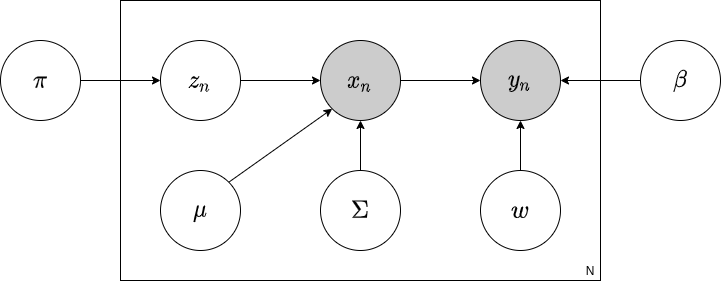
\includegraphics[width=\textwidth]{figure.png} % first figure itself
        \caption{Pictorial Representation of the Generative Story}
    \end{minipage}\hfill
\end{figure}
Part-1: \\

Let $\boldsymbol\Theta = \{\pi_k,\mu_k,\Sigma_k,\vw_k\}_{k=1}^K$\\

The CLL:
\[
\log p (\vX, \vy, \vZ | \boldsymbol\Theta) = \log p (\vy | \vX,\vW, \beta) + \log p (\vX | \vZ, \mu, \Sigma) + \log p (\vZ | \boldsymbol\pi)
\]
Assuming iid variables and substituting their expressions in the CLL we get:
\[
CLL(\vX,\vy,\vZ,\boldsymbol\Theta)=\sum_{n=1}^N\sum_{k=1}^Kz_{nk}\left[-\frac{\beta}{2}(\vy_n-\vw_k^T\vx_n)^2-\frac{1}{2}\log|\boldsymbol\Sigma_k|-\frac{1}{2}(\vx_n-\boldsymbol\mu_k)^T\boldsymbol\Sigma_k^{-1}(\vx_n-\boldsymbol\mu_k)+\log\pi_k\right]
\]
Moving on to the EM algorithm:\\

E-step: \\
\[
\bE[z_{nk}]\propto p(z_{nk}=1|\vx_n,\vy_n,\boldsymbol\Theta)={p(z_n=k|\boldsymbol\pi)p(\vx_n|z_n=k,\boldsymbol\mu_k,\boldsymbol\Sigma_k)}p(\vy_n|\vx_n,z_{nk}=1)
\]
\[
\therefore\bE[z_{nk}]\propto \pi_k N(\vx|\boldsymbol\mu_k,\boldsymbol\Sigma_k) N(\vy_n|\vw_k^T\vx_n,\beta^{-1})
\]
\[
\therefore\bE[z_{nk}]= \frac{\pi_k N(\vx|\boldsymbol\mu_k,\boldsymbol\Sigma_k) N(\vy_n|\vw_k^T\vx_n,\beta^{-1})}{\sum_{k=1}^K\pi_k N(\vx|\boldsymbol\mu_k,\boldsymbol\Sigma_k) N(\vy_n|\vw_k^T\vx_n,\beta^{-1})}
\]
M-step:\\

The objective function is:
\[
\boldsymbol\Theta_{opt}=\underset{\boldsymbol\pi\geq0}{\mathrm{arg max}}=\sum_{n=1}^N\sum_{k=1}^K\bE[z_{nk}]\left[-\frac{\beta}{2}(\vy_n-\vw_k^T\vx_n)^2-\frac{1}{2}(\vx_n-\boldsymbol\mu_k)^T\boldsymbol\Sigma_k^{-1}(\vx_n-\boldsymbol\mu_k)-\frac{1}{2}\log|\boldsymbol\Sigma_k|+\log\pi_k\right]
\]
with the constraint $\sum_{k=1}^K\pi_k=1$.\\

In order to deal with the constraint, we can construct a Lagrangian:
\[
\cL(\boldsymbol\Theta,\boldsymbol\alpha,\theta)=\bE[CLL(\vX,\vy,\vZ,\boldsymbol\Theta)]+\sum_{k=1}^K\alpha_k\pi_k-\theta\left(1-\sum_{k=1}^K\pi_k\right)
\]
\[
\boldsymbol\Theta_{opt}=\underset{}{\mathrm{arg max}}\;\;\underset{\boldsymbol\alpha\geq0}{\mathrm{min}}\;\;\cL(\boldsymbol\Theta,\boldsymbol\alpha,\theta)
\]
On differentiating the Lagrangian w.r.t primal variables we get:
\[
\frac{\partial\cL}{\partial\vw_i}=\beta\vX^Tdiag(\bE[Z_i])(\vy-\vX\vw_i)=0
\]
\[
\implies\vw_i=[\vX^Tdiag(\bE[Z_i])\vX]^{-1}\vX^Tdiag(\bE[Z_i])\vy
\]
where diag($\bE[\vZ_i]$) is a N x N diagonal matrix with $\bE[z_{ji}]$ as the $j^{th}$ diagonal entry.

The expressions obtained for $\mu_i$ and $\sigma_i$ are:
\[
\boldsymbol\mu_i = \frac{1}{N_i}\sum_{n=1}^N\bE[z_{ni}]\vx_n
\]
\[
\boldsymbol\Sigma_i = \frac{1}{N_i}\sum_{n=1}^N\bE[z_{ni}](\vx_n-\boldsymbol\mu_i)(\vx_n-\boldsymbol\mu_i)^T
\]
\[
\frac{\partial\cL}{\partial\pi_i}=\sum_{n=1}^N\frac{\bE[z_{ni}]}{\pi_i}+\alpha_i+\theta=0\implies\pi_i=\frac{N_i}{-\alpha_i-\theta}
\]
where $N_i=\sum_{n=1}^N\bE[z_{ni}]$\\
Formulating the dual and removing unwanted constants we have:
\[
\boldsymbol\alpha_{opt},\theta_{opt}=\underset{\boldsymbol\alpha\geq0}{\mathrm{arg min}} \sum_{n=1}^N\sum_{k=1}^K-\bE[z_{nk}]\log(-\alpha_k-\theta)-\theta
\]
Taking its derivative w.r.t $\alpha_i$ we have:
\[
\frac{\partial\cL}{\partial\alpha_i}=\sum_{n=1}^N\frac{\bE[z_{ni}]}{-\alpha_i-\theta}\geq0
\]
\[\frac{\partial^2\cL}{\partial\alpha_i^2}=\sum_{n=1}^N\frac{\bE[z_{ni}]}{(\alpha_i+\theta)^2}\geq0
\]
Thus, $\cL$ increases monotonically in $\boldsymbol\alpha$, $\boldsymbol\alpha_{opt}=0$
\[
    \therefore\theta = \sum_{n=1}^N\sum_{k=1}^K\bE[z_{nk}]=-N
\]
\[
    \implies\pi_k=\frac{1}{N}\sum_{n=1}^N\bE[z_{ni}]
\]

The EM algorithm can be summarised as follows:

\begin{enumerate}
\item Initialize $\boldsymbol\Theta=\hat{\boldsymbol\Theta}$
\item E-step: Calculate the $\bE[z_{nk}]$ \{for k = 1 to K, n=1 to N\}
\item M-step: Estimate $\boldsymbol\Theta$'s parameters using the expressions given for $\boldsymbol\mu_i,\boldsymbol\Sigma_i,\pi_i$ and $\vw_i$ above \{for k=1 to K\}
\item Go to step-2 if not converged
\end{enumerate}

The expression obtained for weights makes intuitive sense because it is analogous to the weight vector in an importance-weighted linear regression problem. Moreover, if we consider each class as the output of a single regression problem, these expressions start to make intuitive sense.\\

Moving on, for the ALT-OPT algo, we have $\pi_k=\frac{1}{K}$, so $\boldsymbol\Theta=\{\mu_k,\Sigma_k,w_k\}_{k=1}^K$\\

Step-1: MLE estimate of $\vz_n$:
\[
\hat{\vz}_n=\underset{k}{\mathrm{arg max}}\;p(z_n=k|\vX,\vy,\boldsymbol\Theta)\propto p(z_n=k|\boldsymbol\pi)p(\vx_n,\vy_n|z_n=k,\boldsymbol\mu_k,\boldsymbol\Sigma_k)
\]

Transforming it to a minimisation problem and removing constants:
\[
\hat{\vz}_n=\underset{k}{\mathrm{arg min}}[(\vx_n-\boldsymbol\mu_k)^T\boldsymbol\Sigma_k(\vx_n-\boldsymbol\mu_k)+\log|\boldsymbol\Sigma_k|+\frac{\beta}{2}(\vy_n-\vw_k^T\vx_n)^2]
\]

$E[z_{nk}]$ can be replaced by $\hat{z}_{nk}$:
\[
\therefore \boldsymbol\mu_i = \frac{1}{N_i}\sum_{n=1}^N\hat{z}_{ni}\vx_n
\]
\[
\boldsymbol\Sigma_i = \frac{1}{N_i}\sum_{n=1}^N\hat{z}_{ni}(\vx_n-\boldsymbol\mu_i)(\vx_n-\boldsymbol\mu_i)^T
\]
\[
\vw_i=[\vX^Tdiag(\hat{\vZ}_i)\vX]^{-1}\vX^Tdiag(\hat{\vZ}_i)\vy
\]
where $\hat{z}_{nk}=1$ if $\hat{z}_{n}=k$ else 0.

ALT-OPT can be summarised as:
\begin{enumerate}
    \item Initialize $\boldsymbol\Theta=\hat{\boldsymbol\Theta}$
    \item Estimate $\vz_i$ for $i = 1$ to N by solving the minimisation expression shown above.
\item Estimate $\boldsymbol\Theta$ using the expressions given above \{for k = 1 to K\}.
\item Go to step-2 if not converged.
\end{enumerate}

Part-2:\\
Let the params be $\boldsymbol\Theta=\{\boldsymbol\eta_k,\boldsymbol\vw_k\}_{k=1}^K$:\\
Now for the EM, expression for CLL is:
\[
\log p(\vy,\vZ|\vX,\boldsymbol\Theta)=\log p(\vy|\vX,\vW,\beta)+\log p(\vZ|\vX,\boldsymbol\eta)
\]
\[
CLL(\vy,\vZ,\vX,\vTheta)=\sum_{n=1}^N\sum_{k=1}^Kz_{nk}\left[-\frac{\beta}{2}(y_n-\vw^T_K\vx_n)^2+\boldsymbol\eta^T\vx_n-\log\sum_{j=1}^K\exp(\boldsymbol\eta_j^T\vx_n)\right]
\]
For the expectation step:
\[
\bE[z_{nk}]=\frac{\sum_{k=1}^Kz_{nk}p(z_n=k|\vX,\boldsymbol\Theta)}{\sum_{k=1}^Kp(z_n=k|\vX,\boldsymbol\Theta)}=\frac{\sum_{k=1}^Kz_{nk}\pi_k(\vx_n)}{\sum_{k=1}^K\pi_k(\vx_n)}
\]
\[
\implies \bE[z_{nk}]=\frac{\exp(\boldsymbol\eta_k^T\vx_n)}{\sum_{k=1}^K\exp(\boldsymbol\eta_k^T\vx_n)}
\]
For the maximization step, the objective is:
\[
\boldsymbol\Theta_{opt}=\bE[CLL(\vy,\vZ,\vX,\vTheta)]=\sum_{n=1}^N\sum_{k=1}^K\bE[z_{nk}]\left[-\frac{\beta}{2}(y_n-\vw^T_K\vx_n)^2+\boldsymbol\eta^T\vx_n-\log\sum_{j=1}^K\exp(\boldsymbol\eta_j^T\vx_n)\right]
\]

This gives us an unconstrained problem, which can be solved by differentiating:
\[
\vw_i=[\vX^Tdiag(\hat{\vZ}_i)\vX]^{-1}\vX^Tdiag(\hat{\vZ}_i)\vy
\]
\[
\frac{\partial\cL}{\partial\boldsymbol\eta_i}=\sum_{n=1}^N\bE[z_{ni}]\left[\vx_n-\frac{\vx_n\exp(\boldsymbol\eta_i^T\vx_n)}{\sum_{j=1}^K\exp(\boldsymbol\eta_j^T\vx_n)}\right]=0
\]   
\[
\therefore\sum_{n=1}^N\frac{\bE[z_{ni}]\exp(\boldsymbol\eta_i^T\vx_n)}{\sum_{j=1}^K\exp(\boldsymbol\eta_j^T\vx_n)}=\sum_{n=1}^N\bE[z_{ni}]\vx_n
\]
This gives us a system of K non-linear equations for each (i=1,...,K), solving which will give the required $\boldsymbol\eta_i$. It is not possible to get a closed form expression for $\boldsymbol\eta_i$ as they are dependent on each other's value.
\end{mlsolution}
    

\end{document}
